\documentclass{article}
\usepackage[paperwidth=6in, paperheight=9in, margin=0.75in]{geometry}
\usepackage{fontspec}
\usepackage{xcolor}
\usepackage{graphicx}
\usepackage{tikz}

% Set up fonts
\setmainfont[Script=Devanagari] {Tiro Devanagari Marathi}
\newfontfamily\devanagarifont[Scale=MatchUppercase]{Tiro Devanagari Marathi}
%\setmainfont[Script=Devanagari]{Nirmala Text}
%\newfontfamily\devanagarifont[Scale=MatchUppercase]{Nirmala Text}
% \setmainfont[Script=Devanagari]{Noto Serif Devanagari}
% \newfontfamily\devanagarifont[Scale=MatchUppercase]{Noto Serif Devanagari}

\newfontfamily\devtransl[Mapping=DevRom]{Segoe UI}
\graphicspath{{images/}}

% Define colors
\definecolor{titleorange}{RGB}{255,140,0}
\definecolor{subtitleblue}{RGB}{0,51,102}
\definecolor{authorgreen}{RGB}{0,102,51}

\pagestyle{empty}

\begin{document}

% FRONT COVER PAGE
\thispagestyle{empty}
\null\vfill

\begin{center}
% Title - big orange font, 60% page width
{\fontsize{58}{78}\selectfont\color{titleorange}\textbf{व्यूहरूपे}}

\vspace{1em}

% Subtitle - quarter size, dark blue
{\fontsize{12}{14}\selectfont\color{subtitleblue}(रोजच्या जगण्यातील खेळांचे व्यूहशास्त्र)}

\vspace{5em}

% Author - dark green
{\fontsize{16}{20}\selectfont\color{authorgreen}\textbf{डॉ. योगेश हरिभाऊ कुलकर्णी}}
\end{center}

\vfill\null
\clearpage

% BACK COVER PAGE
\thispagestyle{empty}
\vspace*{0.5in}

% Book description
\noindent\textbf{पुस्तकाविषयी:} आपण रोज असंख्य निर्णय घेतो — नोकरीत वाटाघाटी, बाजारात घासाघीस, कार्यालयातील राजकारण, रस्त्यावरील रहदारी. हे सारे एक प्रकारचे खेळ आहेत — जिथे आपला फायदा इतरांच्या निर्णयांवर अवलंबून असतो. ‘व्यूहरूपे’ हे पुस्तक या खेळांचे व्यूहशास्त्र सोप्या, रोचक भाषेत मांडते. गणित नाही, किचकट सिद्धांत नाही, फक्त रोजच्या जगण्यातील उदाहरणे आणि त्यांतून मिळणारे व्यावहारिक धडे. खेळ सिद्धांत (Game Theory) ही एक जीवनदृष्टी आहे — आणि ती एकदा समजली की जग वेगळेच दिसते.

\vspace{1.5em}

% Target audience
\noindent\textbf{वाचकांविषयी:} नोकरदार, उद्योजक, विद्यार्थी आणि रोजच्या जगण्यात चाणाक्षपणे विचार करू इच्छिणाऱ्या सर्वांसाठी.

\vspace{1.5em}

% Author bio
\noindent\textbf{लेखकाविषयी: डॉ. योगेश हरिभाऊ कुलकर्णी} हे कृत्रिम बुद्धिमत्ता, डेटा सायन्स आणि व्यूहरचना या क्षेत्रांतील अनुभवी अभ्यासक व सल्लागार आहेत. दै. सकाळमध्ये ते नियमितपणे तंत्रज्ञान व व्यूहरचना विषयक लेखन करतात. `AI-रूपे’ हे त्यांचे मराठीतील पहिले पुस्तक. TEDx वक्ते. अधिक माहितीसाठी: linkedin.com/in/yogeshkulkarni

\vfill

% Author photo and contact info at bottom
\begin{tabular}{@{}p{0.3\textwidth}@{}p{0.2\textwidth}@{}p{0.3\textwidth}@{}}
\centering
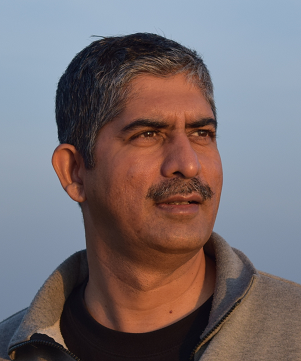
\includegraphics[width=\linewidth,keepaspectratio]{myphoto} 

yogeshkulkarni@yahoo.com
&
% blank column &
& 
\centering

\includegraphics[width=\linewidth,keepaspectratio]{mylinkedinqr}

+91 9890251406
\end{tabular}


% Publisher info at bottom
\begin{center}
\textbf{\ldots} \\ % प्रकाशक: सकाळ प्रकाशन (TBD)
% ISBN-13: (TBD)
\end{center}

\begin{center}

\includegraphics[width=3cm]{isbn_barcode}
\end{center}

\end{document}